\documentclass{article}
\usepackage{amssymb}
\usepackage{xstring}
\usepackage{amsmath}
\newcounter{subjto}
\let\oldsum\sum
\renewcommand{\sum}{\oldsum\limits}
\newcommand{\maxf}[2]{\underset{#1}{\text{maximize}}&&#2}
\newcommand{\minf}[2]{\underset{#1}{\text{minimize}}&&#2}
\newcommand{\con}[2][]{
    \ifnum \value{subjto}>0
    \setcounter{subjto}{0}
    \\
    \text{subject to}
    \else
    ,
    \\
    \fi
    \IfSubStr{#2}{\mathbb{Z}}{
        &\hspace{0.3in}& \StrBefore{#2}{\in} & \in & \mathbb{Z}
        }{
        \IfSubStr{#2}{=}{
            &\hspace{0.3in}& \StrBefore{#2}{=} & = & \StrBehind{#2}{=}
            }{\IfSubStr{#2}{\le}{
                &\hspace{0.3in}& \StrBefore{#2}{\le} & \le & \StrBehind{#2}{\le}
                }{\IfSubStr{#2}{\ge}{
                    &\hspace{0.3in}& \StrBefore{#2}{\ge} & \ge & \StrBehind{#2}{\ge}
                    }{\IfSubStr{#2}{\in}{
                        &\hspace{0.3in}& \StrBefore{#2}{\in} & \in & \StrBehind{#2}{\in}
                        }{
                        error
                    }
                }
            }
        }
    }
    \IfStrEq{#1}{}{
        %        &\hspace{0.3in}& 
        } {
        ,&\hspace{0.3in}& \forall #1
    }
    
}
\newenvironment{mbol}
{
    \setcounter{subjto}{1}
    \begin{equation*}
        \begin{array}{ccrclcl}
        }
        {
            .\\
        \end{array}
    \end{equation*}
}

\usepackage{amssymb}
\usepackage{xstring}
\usepackage{amsmath}
\usepackage{verbatim}
\usepackage{graphicx}
\usepackage{listings}
\usepackage{color} \usepackage{transparent}

\newcommand{\subheader}[1]{
    \vspace{0.5in}
    \noindent\textbf{#1}:
}

\newcommand{\mboldescrip}[5]{
    \subheader{#1}
    \begin{itemize}
        \item Latex: \texttt{#2}
        \item Mathematical notation: #3
        \item Description: #4
        \item Example: #5
    \end{itemize}
}

\newcommand{\hil}[1]{\textcolor{red}{#1}}

\begin{document}

\title{Math-Based Optimization Language (MBOL)}

\author{Andrew Newell}

\maketitle

\tableofcontents

\section{Introduction}

This document should explain the MBOL language which is a subset of the Latex language. The goal is to convert natural mathematical representations of optimization programs into a solver. Currently MBOL supports linear programs or mixed integer programs.

\begin{figure}
    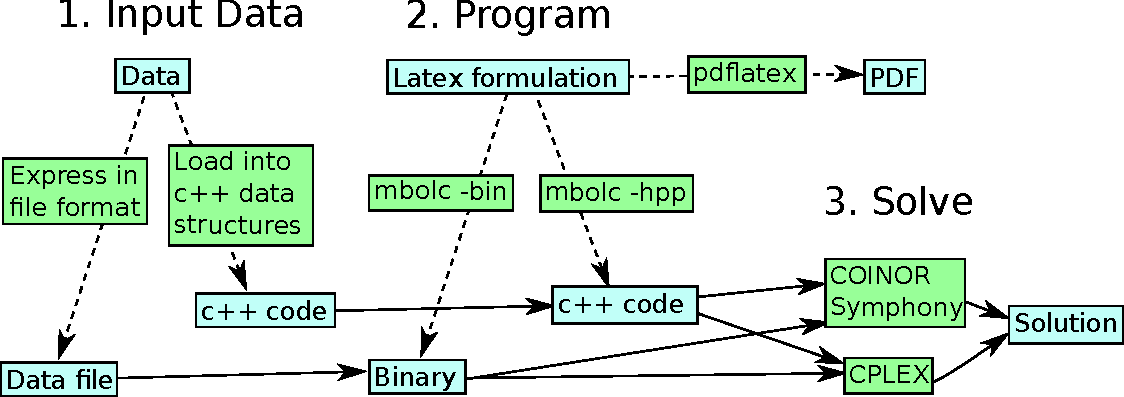
\includegraphics[width=\textwidth]{figures/mbol-overview.pdf}
    \caption{Overview of workflow using MBOL}
    \label{lab:overview}
\end{figure}

Figure~\ref{lab:overview} shows an overview of MBOL. The goal is to automate and simplify the implementation of optimization programs.

\section{Getting Started}

The best flow to get started is to compile the code, setup your environment, and try out the sample programs.

\subsection{Compiling}

\subheader{Requirements} yacc, lex, and g++ which are all common utilities especially for compiling compilers.

\subheader{Compile} Execute \texttt{make} in the top-level directory. The resulting binary \texttt{mbolc} (MBOL compiler), will be in the \texttt{bin} directory.

\subheader{Install} Execute \texttt{sudo make install} if you would like \texttt{mbolc} to be added to /usr/bin.

\subsection{Environment setup}

The MBOL compiler creates code that requires files in the include directory. In the top-level directory execute the following:
\begin{verbatim}
    export MBOL_HOME=`pwd`
\end{verbatim}
You may want to add some equivalent of this in your \texttt{.bashrc}. This can be added automatically by typing \texttt{make env} in the top-level directory. You will need to invoke \texttt{source ~/.bashrc} or load a new shell.

Currently, we support solving with CPLEX through their Concert API or any other solver that can read the mixed integer program format \texttt{.mps}. To solve with CPLEX through Concert, you must setup the \texttt{CPLEX\_HOME} environment variable to point to CPLEX's home directory. For other solvers, e.g. \texttt{symphony}, you need to ensure the executable that solves a given \texttt{.mps} is available to be invoked.

\subsection{Sample programs}

Sample programs are provided in the \texttt{samples} directory. Type \texttt{make} to create code, \texttt{./main} to try running the code, and \texttt{make svm} to create some visuals based on the SVM part of the sample code. 

After compiling, notice that the pdf directory contains the pdf versions of each mbol-source file. By understanding how things were built here, much of mbolc can be understood to see how to create code, pdfs, and binaries. 

A binary is created in the maxflow directory for one particular problem. The binary requires no c++ code for data input, but it requires a special input file format shown in this maxflow directory.

\section{MBOL Language}

The language for MBOL is a subset of the Latex language. Latex is the standard for nearly any commonly used mathematical notation. MBOL is a subset of mathematical notation which is already commonly used to describe optimization problems. By specifying this strict subset of the language, MBOL syntax can be compiled into an optimization program that can be used by various state-of-the-art solvers.

The goal here is to describe the details of the grammar of the language. The full grammar is included in this directory under mbol-grammar.txt which is comprehensive as it is automatically generated, but this full grammar does not explain how the grammar affects the optimization programs.


We will focus on a well-known problem of vertex cover which can be expressed in latex as follows:

\begin{verbatim}
    \begin{mbol}
        \minf{x}{\sum_{v \in V} x_v}
        \con[(u, v) \in E]{x_u + x_v \ge 1}
        \con[v \in V]{x_v \in \{0,1\}}
    \end{mbol}
\end{verbatim}

The programs are described with a series of MBOL latex commands \texttt{\textbackslash maxf}, \texttt{\textbackslash minf}, and \texttt{\textbackslash con} for maximum objective, minimum objective, and constraint respectively. These commands help create an unamibiguous language which is compiled to be solved. Additionally, these commands perform nice optimization typesetting, seen in the following:

\begin{mbol}
    \minf{x}{\sum_{v \in V} x_v}
    \con[(u, v) \in E]{x_u + x_v \ge 1}
    \con[v \in V]{x_v \in \{0,1\}}
\end{mbol}

To those familiar with optimization programs, this format is perfectly understandable and unambiguous. The goal of MBOL is to formally specify the language, and then automatically use this formulation to solve. This program will be disected, to describe what each part means mathematically. We note that the only input to the compiler is the above MBOL source, everything below about variables and constraints is inferred from the grammar.

\subsection{Variables}

\subheader{Program variables}

\begin{mbol}
    \minf{\hil{x}}{\sum_{v \in V} x_v}
    \con[(u, v) \in E]{x_u + x_v \ge 1}
    \con[v \in V]{x_v \in \{0,1\}}
\end{mbol}

The x under the minimize (or maximize), are variables of the program. All other variables are either temporaries or constants. We borrow these notions of variables from standard computer programming, but they have mathematical meaning which is not usually explicitly described.

\subheader{Program temporaries}

\begin{mbol}
    \minf{x}{\sum_{\hil{v} \in V} x_{\hil{v}}}
    ,\\&\hspace{0.3in}& x_{\hil{u}} + x_{\hil{v}} & \ge & 1 ,&\hspace{0.3in}& \forall (\hil{u}, \hil{v}) \in E
    ,\\&\hspace{0.3in}& x_{\hil{v}} &\in& \{0,1\} ,&\hspace{0.3in}& \forall \hil{v} \in V
\end{mbol}

The u and v variables in this program are temporaries. They are described as elements of a set. Their purpose can either be to express a set of values for a sum or a set of inequalities for constraints. Temporaries are inferred by the grammar of MBOL.

\subheader{Program constants}

\begin{mbol}
    \minf{x}{\sum_{v \in \hil{V}} x_v}
    ,\\&\hspace{0.3in}& x_u + x_v & \ge & 1 ,&\hspace{0.3in}& \forall (u, v) \in \hil{E}
    ,\\&\hspace{0.3in}& x_v &\in& \{0,1\} ,&\hspace{0.3in}& \forall v \in \hil{V}
\end{mbol}

These variables are constants, which are inferred by the grammar as well. They are those variables left over that are neither program variables nor temporaries. The constants are the inputs to the program while the objective value and values of the program variables are output.

In addition to whether a variable is a program variable, program temporary, or program constant, the variables have another distinction based on their type as a number or and element described as follows:

\subheader{Variable type, elements}

\begin{mbol}
    \minf{x}{\sum_{\hil{v} \in \hil{V}} x_{\hil{v}}} 
    ,\\&\hspace{0.3in}& x_{\hil{u}} + x_{\hil{v}} & \ge & 1 ,&\hspace{0.3in}& \forall (\hil{u}, \hil{v}) \in \hil{E}
    ,\\&\hspace{0.3in}& x_{\hil{v}} &\in& \{0,1\} ,&\hspace{0.3in}& \forall \hil{v} \in \hil{V}
\end{mbol}

These are elements in this program. An element is an integer, set of elements, or set of tuples. There is a lot of recursive possibilities here which is intentional. Also, these types are not supplied by the user, they are all inferred by the grammar. The inference creates a graph based with edges that define relationships between elements. In this program, the elements have the following types and meaning in terms of the graph used for vertex cut:
\begin{itemize}
    \item $v$: integer (single vertex)
    \item $u$: integer (single vertex)
    \item $V$: set of integers (vertices)
    \item $E$: set of tuples where each tuple has two integers (edges)
\end{itemize}

\subheader{Variable type, numbers}

\begin{mbol}
    \minf{\hil{x}}{\sum_{v \in V} \hil{x_v}}
    ,\\&\hspace{0.3in}& \hil{x_u} + \hil{x_v} & \ge & 1 ,&\hspace{0.3in}& \forall (u, v) \in E
    ,\\&\hspace{0.3in}& \hil{x_{v}} &\in& \{0,1\} ,&\hspace{0.3in}& \forall v \in V
\end{mbol}

The other variable type are simply numbers. These are initially assumed to be unbounded real numbers until constraints are placed on them. In this case, the variable $x$ is constrained to be a binary variable. Numbers can be indexed, so they behave similar to a map in computer programming. In this case $x$ has one integer index, so it has a separate integer value $x_v$ for each integer $v$ used as an index. Note that indices must be elements, and these elements can be very complicated. In this program nothing would prevent a new number variable $y$ being used indexed by $y_E$ meaning that it is indexed by a set of 2-tuples. These cases seem strange, but in combinatorial optimization they can be incredible powerful in describing realistic problems.

\begin{mbol}
    \minf{x}{\sum_{v \in V} x_v}
    \con[(u, v) \in E]{x_u + x_v \ge 1}
    \con[v \in V]{x_v \in \{0,1\}}
\end{mbol}

\section{Additional grammar features}

\mboldescrip{Strict subset}{X \textbackslash subset Y}{$X \subset Y$}{Creates all possible subsets for summations or constraints}{$Y=\{1,2,3\}$ implies that we get the following 7 sets $X=\{\},\{1\},\{2\},\{3\},\{1,2\},\{1,3\},\{2,3\}$}

\mboldescrip{Subset}{X \textbackslash subseteq Y}{$X \subseteq Y$}{Creates all possible subsets for summations or constraints}{$Y=\{1,2,3\}$ implies that we get the following 8 sets $X=\{\},\{1\},\{2\},\{3\},\{1,2\},\{1,3\},\{2,3\},\{1,2,3\}$}

\mboldescrip{Integer constraint}{x \textbackslash in \textbackslash mathbb\{Z\}}{$x\in \mathbb{Z}$}{Variable $x$ is constrained to be an integer variable}{$x \in \mathbb{Z}$ implies $x = ...,-2,-1,0,+1,+2,...$}

\mboldescrip{Comparison operators}{= $<$ $>$ \textbackslash le \textbackslash ge}{$= < > \le \ge$}{Constraint operatorst which could constrain the program or even a constraint placed on variables of a summation or constraint set}{Standard equality/inequality operators}

\mboldescrip{Tuple}{(i, j, k)}{$(i,j,k)$}{Tuple of elements, where each element could be a set, tuple, or integer}{$(i,j,k)$ is a 3-tuple, where $i$ could be a set $i=\{1,2\}$, $j$ could be another tuple with two integers $j=(5,7)$, and $k$ could be a simple integer $k=2$}

\mboldescrip{Emptyset}{\textbackslash emptyset}{$\emptyset$}{Set with no elements, useful for putting conditions on whether certain constraints or iterations of a summation are used}{$\emptyset \ne S$ implies that $S$ cannot be empty}

\mboldescrip{Counting iteration}{x=a,...,b}{$x=a,...,b$}{Iterates from integers $a$ to $b$ counting by 1}{$x=a,...,b$ where $a=2$ and $b=8$ will result in $x=2,3,4,5,6,7,8$}

\mboldescrip{Inequality iteration}{a \textbackslash le x \textbackslash le b}{$a \le x \le b$}{Iterates from integers $a$ to $b$ counting by 1}{$a \le x \le b$ where $a=2$ and $b=8$ will result in $x=2,3,4,5,6,7,8$}

\mboldescrip{Set minus}{X \textbackslash setminus Y}{$X \setminus Y$}{Removes elements of $Y$ from $X$}{$\{1,2,5,6,7\} \setminus \{2,3,4,5\} = \{1,6,7\}$}

\mboldescrip{Set union}{X \textbackslash cup Y}{$X \cup Y$}{Creates the union of sets $Y$ and $X$}{$\{1,2,5,6,7\} \cup \{2,3,4,5\} = \{1,2,3,4,5,6,7\}$}

\mboldescrip{Set intersect}{X \textbackslash cap Y}{$X \cap Y$}{Creates the intersect of sets $Y$ and $X$}{$\{1,2,5,6,7\} \cap \{2,3,4,5\} = \{2,5\}$}

\mboldescrip{Set creator}{\{x : x \textbackslash in Y, x $>$ 5\}}{$\{x : x \in Y, x > 5\}$}{Creates a set with specified qualifiers}{$\{x : x \in \{1,4,5,6,8,9\}, x > 5\}=\{6,8,9\}$}

\mboldescrip{Set}{\{x, y, z\}}{$\{x,y,z\}$}{Creates a set with the elements listed}{$\{x,y,z\}$ is a set of these 3 elements}

\mboldescrip{Cardinality}{$|$ X $|$}{$|X|$}{The number of elements in the set}{$|\{6,7,9\}| = 3$}

\mboldescrip{Exponent}{(x)\^{}\{y\}}{$(x)^{y}$}{Raise a value $x$ to the power $y$}{$(2)^{3}=8$}

\mboldescrip{Fraction}{\textbackslash frac\{x\}\{y\}}{$\frac{x}{y}$}{$x$ divided by $y$}{$\frac{9}{4}=2.25$}

\mboldescrip{Indices}{x\_\{i,j\}}{$x_{i,j}$}{$(i,j)th$ value of $x$}{$x_{i,j}$ could stand for the $i$th row and $j$th column of a matrix}

\mboldescrip{Set summation}{\textbackslash sum\_\{a \textbackslash in S \}(x\_a)}{$\sum_{a \in S}(x_a)$}{Sum all values $x_a$ where $a$ is in $S$}{$\sum_{a \in \{1,5,6,7\}}(x_a) = x_1+x_5+x_6+x_7$}

\mboldescrip{Counting summation}{\textbackslash sum\_\{i = 1\}\^{}\{n\}(x\_i)}{$\sum_{i=1}^{n}(x_i)$}{Sum all values $x_i$ where $1 \le i \le n$}{$\sum_{i=1}^{5}(x_i) = x_1+x_2+x_3+x_4+x_5$}

\end{document}
